\documentclass{article}

\usepackage{pandekten}

\usepackage{dashrule}

\makeatletter
\newcommand*{\shifttext}[1]{%
  \settowidth{\@tempdima}{#1}%
  \hspace{-\@tempdima}#1%
}
\newcommand{\plabel}[1]{%
\shifttext{\textbf{#1}\quad}%
}
\newcommand{\prule}{%
\begin{center}%
\hdashrule[0.5ex]{.99\linewidth}{1pt}{1pt 2.5pt}%
\end{center}%
}

\makeatother

\setlength{\parindent}{0pt}

\title{Assignment 3}
\author{Ze Chen}

\begin{document}

\maketitle

\plabel{1 (1)}%
They applied $V_L$ and $V_R$ to move the energy levels and accomondate $\ket{\downarrow}$ electrons.
\begin{center}
    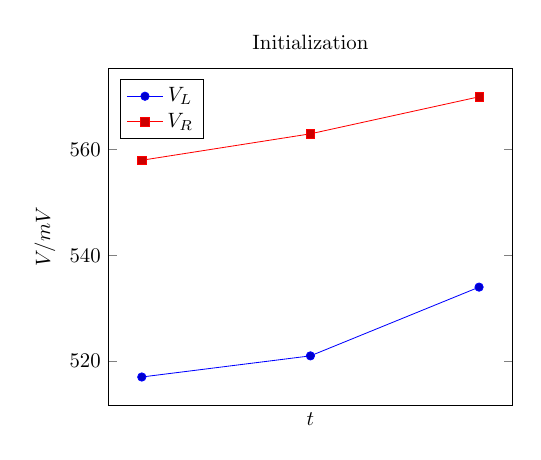
\begin{tikzpicture}[scale=0.75]
        \begin{axis}[title=Initialization,xmajorticks=false,xlabel=$t$,ylabel=$V/\text{mV}$,legend pos=north west]
            \addplot coordinates {
                (0,517) (1,521) (2,534)
            };\addplot coordinates {
                (0,558) (1,563) (2,570)
            };
            \legend{$V_L$,$V_R$}
        \end{axis}
    \end{tikzpicture}
\end{center}
\begin{center}
    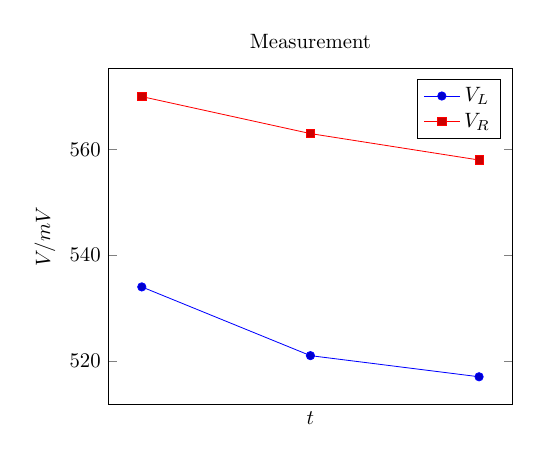
\begin{tikzpicture}[scale=0.75]
        \begin{axis}[title=Measurement,xmajorticks=false,xlabel=$t$,ylabel=$V/\text{mV}$,legend pos=north east]
            \addplot coordinates {
                (0,534) (1,521) (2,517)
            };\addplot coordinates {
                (0,570) (1,563) (2,558)
            };
            \legend{$V_L$,$V_R$}
        \end{axis}
    \end{tikzpicture}
\end{center}

\plabel{(2.a)}%
They introduced a Co micromagnet which generates a magnetic field gradient that results in distinct ESR transition frequencies for the left and right qubits.

\plabel{(2.b)}%
The electric field drives an oscillating electron, which experiences an oscillating magnetic field.
The oscillation has amplitude $\Delta \vb{B} \propto \vb{E}\cdot \grad \vb{B}$.
Therefore, $\grad \vb{B}$ and the magnetic moment determines $\Omega/E$.

\plabel{(3.a)}%
The Hamiltonian is given by
\[ H = \left(
    \begin{array}{cccc}
     B & 0 & 0 & 0 \\
     0 & -\frac{J}{2} & \frac{J}{2} & 0 \\
     0 & \frac{J}{2} & -\frac{J}{2} & 0 \\
     0 & 0 & 0 & -B \\
    \end{array}
    \right).
\]
The eigenvalues are $(-J,0,+B,-B)$.
\begin{center}
    \begin{tikzpicture}
        \begin{axis}[domain=0:10,samples=100,xlabel=$B/J$,ylabel=$E/J$]
            \addplot[] {-1};
            \addplot[] {0};
            \addplot[] {x};
            \addplot[] {-x};
        \end{axis}
    \end{tikzpicture}
\end{center}
With $\delta B$ the Hamiltonian is given by
\[ H = \begin{pmatrix}
    \delta B - J/2 & J/2 \\
    J/2 & -\delta B - J/2
\end{pmatrix}. \]
In the limit $\delta B \gg J$ the eigensystem is just
\begin{align*}
    \ket{+B} &= \ket{\uparrow\uparrow}, \\
    \ket{+\delta B} &= \ket{\uparrow\downarrow}, \\
    \ket{-\delta B} &= \ket{\downarrow\uparrow}, \\
    \ket{-B} &= \ket{\downarrow\downarrow},
\end{align*}
which is identical to the one in Fig. 3A.

\plabel{(3.b)}%
There is no $\ket{\downarrow\uparrow}\rightarrow \ket{\downarrow\downarrow}$ or $\ket{\uparrow\downarrow} \rightarrow \ket{\uparrow\uparrow}$.
$f^L_{\ket{\psi_R}=\ket{\uparrow}}$ corresponds to $E_{\ket{\uparrow\uparrow}} - E_{\ket{\downarrow\uparrow}}$, and
$f^L_{\ket{\psi_R}=\ket{\downarrow}}$ corresponds to $E_{\ket{\uparrow\downarrow}} - E_{\ket{\downarrow\downarrow}}$.

\plabel{(4)}%
They measured single qubit transition frequencies with a Hahn echo sequence.
At $t = \SI{204}{\nano\second}$ they find $P^L_\uparrow = 1- P^R_\uparrow$ in all four cases.
They found the corrected fidelity of the CNOT gate to be \SI{78}{\percent}.

\prule

\plabel{2 (1)}%
The rotation is given by
\[ Y_{\pi/2} = \frac{1}{\sqrt{2}} \begin{pmatrix}
    1 & 1 \\
    -1 & 1
\end{pmatrix}. \]
Therefore, the evolution is given by
\[ \ket{\uparrow} \xrightarrow{Y_{\pi/2}} \frac{1}{\sqrt{2}}(\ket{\uparrow} - \ket{\downarrow}) \xrightarrow{\text{free } \tau} \frac{1}{\sqrt{2}}(\ket{\uparrow} - \ket{\downarrow}) \xrightarrow{Y_{\pi/2}} -\ket{\downarrow}. \]

\plabel{(2)}%
The evolution is given by
\begin{align*}
    \ket{\uparrow} &\xrightarrow{Y_{\pi/2}} \frac{1}{\sqrt{2}}(\ket{\uparrow} - \ket{\downarrow}) \\
    &\xrightarrow{\text{free } \tau} \frac{1}{\sqrt{2}}(\ket{\uparrow} - e^{-i(\delta\omega+\gamma\delta B)\tau}\ket{\downarrow}) \\
    &\xrightarrow{Y_{\pi/2}} \frac{1}{2}\qty(1 - e^{-i(\delta\omega+\gamma\delta B)\tau})\ket{\uparrow} - \frac{1}{2}\qty(1 + e^{-i(\delta\omega+\gamma\delta B)\tau})\ket{\downarrow}.
\end{align*}
Therefore,
\begin{align*}
    P_\uparrow &= \int \dd{(\delta B)} \frac{1}{2}\qty(1 - \cos(\delta\omega\tau+\gamma\delta B \tau)) \frac{1}{\sqrt{2\pi}\sigma_B} e^{-(\delta B)^2 / (2 \sigma^2_B)} \\
    &= \frac{1}{2}\qty(1 - \cos(\tau \delta\omega) e^{-\gamma^2 \sigma_B^2\tau^2/2}).
\end{align*}
From Fig. 2b we find $\delta\omega = \SI{29}{\kilo\hertz}$.
Since $\gamma^2 \sigma_B^2 T_{2e}^2 / 2 = \ln 2$ where $\gamma = 2\pi \times \SI{28}{\giga\hertz/\tesla}$ and $T_{2e} = \SI{268}{\micro\second}$ we find $\sigma_B = \SI{25}{\nano\tesla}$.

\plabel{(3)}%
The rotation by $\pi$ is given by
\[ Y_\pi = \begin{pmatrix}
    & 1 \\ -1
\end{pmatrix}. \]
The evolution is given by
\begin{align*}
    \ket{\uparrow} &\xrightarrow{Y_{\pi/2}} \frac{1}{\sqrt{2}}(\ket{\uparrow} - \ket{\downarrow}) \\
    &\xrightarrow{\text{free } \tau/2} \frac{1}{\sqrt{2}}(\ket{\uparrow} - e^{-i(\delta\omega+\gamma\delta B)\tau/2}\ket{\downarrow}) \\
    &\xrightarrow{Y_\pi} \frac{1}{\sqrt{2}}(-e^{-i(\delta\omega+\gamma\delta B)\tau/2} \ket{\uparrow} - \ket{\downarrow}) \\
    &\xrightarrow{\text{free } \tau/2} \frac{1}{\sqrt{2}}e^{-i(\delta\omega+\gamma\delta B)\tau}(-\ket{\uparrow} - \ket{\downarrow}) \\
    &\xrightarrow{Y_{\pi/2}} -e^{-i(\delta\omega+\gamma\delta B)\tau}\ket{\uparrow}.
\end{align*}
Therefore, $P_\uparrow = 1$.
$P_\uparrow$ still decays because $\delta B$ varies with time and is not completely static.
In Fig. 2e there are more $Y_\pi$ applied and therefore the elimination of relative phase shift happens more frequently.

\plabel{(4)}%
The dephasing time is most relevant.
It measures the quality of a single qubit.

\plabel{(5)}%
The ratio of Hahn-echo times for electrons and bare nucleus is close to the ratio of their $\gamma$ factors (\num{1623}) and therefore smaller magnetic moment may play a role here.

% \bibliographystyle{plain}
% \bibliography{main}

\end{document}
